\documentclass[a4paper, czech]{article}

\usepackage[czech]{babel}
\usepackage{indentfirst}
\usepackage{graphicx}
\usepackage{float}
\usepackage[margin=1.5cm]{geometry}
\usepackage{booktabs}
\usepackage{amsmath}
\usepackage[table]{xcolor}
\usepackage{multirow}
\usepackage{tabularray}
\usepackage{bold-extra}


\begin{document}
\begin{table}[H]
    \centering
    \begin{tblr}{
        cell{1}{1} = {c = 2, r = 4}{c}, % Logo
        cell{1}{4} = {c = 3}{c}, % Předmět
        cell{2}{4} = {c = 3}{c}, % Jméno
        cell{3}{4} = {}{c}, % Ročník
        cell{3}{6} = {}{c}, % Studijní skupina
        cell{4}{4} = {}{c}, % Spolupracoval
        cell{4}{6} = {}{c}, % Mereno dne
        cell{5}{1} = {c = 2}{55mm}, % Kontroloval
        cell{5}{3} = {c = 2}{55mm}, % Hodnoceni
        cell{5}{5} = {c = 2}{55mm}, % Dne
        cell{6}{2} = {c = 5}{}, % Nazev ulohy
        cell{7}{1} = {}{c}, % Číslo úlohy
        cell{7}{2} = {c = 5}{c}, % Název úlohy
        vline{1,2,7} = {1.2pt},
        vline{3,5},
        hline{1,5,6,8} = {1.2pt},
        hline{2,3,4}
        }
        
\includegraphics{logo_fekt.png} & & \textsuperscript{Předmět} & \large \textbf{Měření v audiotechnice} \\
             & & \textsuperscript{Jméno} & \large \textbf{Karolína Šebestová} \\
             & & \textsuperscript{Ročník} & \large \textbf{3.} & \textsuperscript{Studijní skupina} & \large \textbf{St 14:00} \\
             & & \textsuperscript{Spolupracoval} & \large \textbf{Filip Kokavec} & \textsuperscript{Měřeno dne} & \large \textbf{23.10.2024} \\
        \textsuperscript{Kontroloval} & & \textsuperscript{Hodnocení} & & \textsuperscript{Dne} \\
        \textsuperscript{Číslo úlohy} & \textsuperscript{Název úlohy} \\
        \Large \textbf{4} & \Large \textsc{\textbf{Měření napětí neharmonických signálů}} \\
    \end{tblr}
\end{table}

\section{Zadání}

\begin{itemize}
    \item Obeznamte se s vlivem kmitočtu a tvaru signálu na přesnost měření efektivní hodnoty
    napětí běžnými měřicími přístroji.
    \item Změřte kmitočtové závislosti:
    \begin{itemize}
        \item číslicového voltmetru s převodníkem skutečné efektivní hodnoty,
        \item číslicového voltmetru s převodníkem střední absolutní hodnoty,
        \item analogového magnetoelektrického voltmetru s operačním usměrňovačem,
        \item analogového magnetoelektrického voltmetru s pasivním usměrňovačem.
    \end{itemize}
    \item Změřte efektivní hodnoty napětí signálu trojúhelníkového a obdélníkového průběhu
    pro zadaný kmitočet základní harmonické složky a stanovte relativní odchylku
    metody.
    \item Změřte efektivní hodnoty napětí signálů vzniklých superpozicí stejnosměrné složky
    a napětí harmonického, trojúhelníkového a obdélníkového průběhu a stanovte relativní
    odchylku metody.
    \item Změřte efektivní hodnoty napětí obdélníkového průběhu pro zadaný kmitočet
    s rozdílnou velikostí střídy a stanovte relativní odchylku metody.
\end{itemize}

\section{Teoretický úvod}

Efektivní hodnota je označení pro energetický obsah napětí.
Je definována vztahem:
\begin{equation*}
    U = \sqrt{\frac{1}{T} \int_0^T u^2\left(t\right) dt}
\end{equation*}

Skutečnou efektivní hodnotu měří analogové přístroje feromagnetické, elektrodynamické, elektrostatické a magnetoelektrické s termočlánkem.
Mezi digitálními pak ty s označením TRMS (True Root Mean Square).
Osciloskopy pro měření používají rozklad na Fourierovu řadu a efektivní hodnotu pak vyjadřují podle vztahu:
\begin{equation*}
    U = \sqrt{U_S^2 + \sum_{k=1}^{\infty} U_k^2}
\end{equation*}
kde Us je stejnosměrnou složkou, Uk střídavá složka a k značí k-tou harmonickou složku.

Většina přístrojů filtruje stejnosměrnou složku oddělovacím kondenzátorem a propouští pouze střídavou složku efektivní hodnoty.
Uvažujeme-li konečný počet harmonických složek N:
\begin{equation*}
    U \left(N\right) = \sqrt{U_S^2 + \sum_{k=1}^{N} U_k^2}
\end{equation*}

Relativní odchylka v závislosti na počtu harmonických složek je definována vztahem:
\begin{equation*}
    \delta_U \left(N\right) = \frac{U \left(N\right) - U}{U} \cdot 100\%
\end{equation*}

Přístroje jsou obvykle kalibrovány pro referenční kmitočet 50 Hz. Kmitočtová závislost je definována vztahem:
\begin{equation*}
    A \left(f\right) = \frac{U\left(f\right)}{U\left(50\right)}
\end{equation*}
kde $U\left(f\right)$ je hodnota na přístroji při kmitočtu $f$.

Existují také přístroje, které měří střední absolutní hodnotu.
Jsou to magnetoelektrické s usměrňovači a také levnější číslicové.
Střední absolutní hodnota je definována vztahem:
\begin{equation*}
    U_{sa} = \frac{1}{T} \int_{0}^{T} \left|u\left(t\right)\right| dt
\end{equation*}
Pro kmitočty, ve kterých přístroje nejsou nekalibrovány udává výrobce odchylku pro určité rozsahy. 

Některé přístroje se pro měření efektivní hodnoty přímo nehodí, můžeme ale využít vztahu:
\begin{equation*}
    U = \sqrt{U_S^2 + U_{\sim}^2}
\end{equation*}
$U_S$ je zde stejnosměrnou složkou a $U_{\sim}$ je složka střídavá.

\begin{figure}[H]
    \centering
    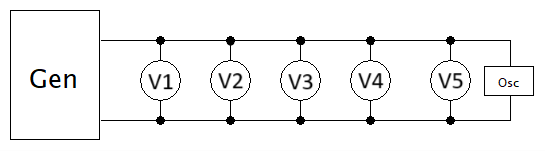
\includegraphics[width=0.4\textwidth]{schema1.png}
    \caption{Schéma zapojení pracoviště při měření voltmetry}
\end{figure}

\section{Výsledky měření}

\subsection{Tabulky}

\begin{table}[H]
    \catcode`\-=12
    \centering
    \caption{Měření kmitočtových závislostí přístrojů}
    \begin{tabular}{ccccccccc}
        \toprule
        $f$      & $U_1$    & $A_1$    & $U_2$   & $A_2$    & $U_3$  & $A_3$    & $U_4$   & $A_4$    \\
        \cmidrule(rl){1-1}
        \cmidrule(rl){2-3}
        \cmidrule(rl){4-5}
        \cmidrule(rl){6-7}
        \cmidrule(rl){8-9}
        Hz     & V     & -     & V    & -     & V   & -     & V    & -     \\
        \midrule
        10     & 5,003 & 0,996 & 5,05 & 1,010 & 4,8 & 1,000 & 4,90 & 1,021 \\
        20     & 5,012 & 0,998 & 5,01 & 1,002 & 4,8 & 1,000 & 4,85 & 1,010 \\
        50     & 5,021 & 1,000 & 5,00 & 1,000 & 4,8 & 1,000 & 4,80 & 1,000 \\
        100    & 5,028 & 1,001 & 5,00 & 1,000 & 4,8 & 1,000 & 4,80 & 1,000 \\
        200    & 5,031 & 1,002 & 5,00 & 1,000 & 4,8 & 1,000 & 4,80 & 1,000 \\
        500    & 5,032 & 1,002 & 4,99 & 0,998 & 4,8 & 1,000 & 4,80 & 1,000 \\
        1000   & 5,030 & 1,002 & 4,98 & 0,996 & 4,8 & 1,000 & 4,80 & 1,000 \\
        2000   & 5,022 & 1,000 & 4,92 & 0,984 & 4,6 & 0,958 & 4,80 & 1,000 \\
        5000   & 4,996 & 0,995 & 4,61 & 0,922 & 4,4 & 0,917 & 4,80 & 1,000 \\
        10000  & 4,976 & 0,991 & 3,82 & 0,764 & 4,2 & 0,875 & 4,80 & 1,000 \\
        20000  & 4,976 & 0,991 & 2,42 & 0,484 & 4,0 & 0,833 & 4,80 & 1,000 \\
        50000  & 5,105 & 1,017 & 0,64 & 0,128 & 2,4 & 0,500 & 4,60 & 0,958 \\
        100000 & 5,688 & 1,133 & 0,15 & 0,030 & 0,6 & 0,125 & 4,00 & 0,833 \\
        \bottomrule
        \multicolumn{9}{l}{$U = 5V$}
    \end{tabular}
\end{table}

\begin{table}[H]
    \catcode`\-=12
    \centering
    \caption{Měření napětí trojúhelníkového a obdélníkového průběhu}
    \begin{tabular}{cccccccccccc}
        \toprule
        \multirow{2}{*}{Průběh} & $k_t$    & $U_1$    & $\delta_1$    & $U_2$    & $\delta_2$     & $U_{2k}$   & $\delta_{2k}$    & $U_3$    & $\delta_3$     & $U_{3k}$   & $\delta_{3k}$    \\
        \cmidrule(rl){2-2}
        \cmidrule(rl){3-4}
        \cmidrule(rl){5-8}
        \cmidrule(rl){9-12}
                                & -     & V     & \%    & V     & \%     & V     & \%     & V     & \%     & V     & \%     \\
        \midrule
        Trojúhelník             & 1,155 & 5,022 & 0,440 & 4,810 & -3,800 & 5,000 & 0,010  & 4,600 & -8,000 & 4,782 & -4,356 \\
        Obdélník                & 1,000 & 5,029 & 0,580 & 5,540 & 10,80  & 4,986 & -0,270 & 5,200 & 4,000  & 4,680 & -6,391 \\
        \bottomrule
        \multicolumn{12}{l}{$U = 5V;\ f = 50 Hz$}
    \end{tabular}
\end{table}

\begin{table}[H]
    \catcode`\-=12
    \centering
    \caption{Měření s nenulovou stejnosměrnou složkou}
    \begin{tabular}{ccccccccccc}
        \toprule
        \multirow{2}{*}{Průběh} & $U_1$    & $\delta_1$    & $U_2$    & $\delta_2$     & $U_{2k}$   & $\delta_{2k}$    & $U_3$    & $\delta_3$     & $U_{3k}$   & $\delta_{3k}$    \\
        \cmidrule(rl){2-3}
        \cmidrule(rl){4-7}
        \cmidrule(rl){8-11}
                                & V     & \%     & V    & \%     & V     & \%     & V   & \%     & V     & \%     \\
        \midrule
        Harmonický              & 4,036 & -19,60 & 4,04 & -19,62 & 4,035 & -19,62 & 4,2 & -16,33 & 4,587 & -8,623 \\
        Trojúhelníkový          & 4,012 & -20,08 & 3,86 & -23,11 & 3,874 & -22,83 & 4,0 & -20,32 & 4,376 & -12,82 \\
        Obdélníkový             & 4,056 & -19,20 & 4,47 & -10,96 & 4,023 & -19,85 & 4,2 & -16,33 & 4,725 & -5,867 \\
        \bottomrule
        \multicolumn{11}{l}{$U_{\sim} = 4V;\ U_s = 3V;\ f = 50 Hz;\ U_R = 5,02V$}
    \end{tabular}
\end{table}

\begin{table}[H]
    \catcode`\-=12
    \centering
    \caption{Závislost efektivní hodnoty napětí na střídě obdélníkového signálu}
    \begin{tabular}{cccccc}
        \toprule
        střída & $U_R$    & $U_1$    & $\delta_1$     & $U_{OSC}$ & $\delta_{OSC}$  \\
        \cmidrule(rl){1-1}
        \cmidrule(rl){2-2}
        \cmidrule(rl){3-4}
        \cmidrule(rl){5-6}
        \%     & V     & V     & \%     & V    & \%    \\
        \midrule
        1      & 5,049 & 0,972 & -80,75 & 5,16 & 2,198 \\
        2      & 5,046 & 1,383 & -72,59 & 5,16 & 2,259 \\
        3      & 5,044 & 1,694 & -66,42 & 5,16 & 2,300 \\
        4      & 5,043 & 1,953 & -61,27 & 5,15 & 2,122 \\
        5      & 5,041 & 2,176 & -56,83 & 5,15 & 2,162 \\
        6      & 5,039 & 2,376 & -52,85 & 5,15 & 2,203 \\
        7      & 5,038 & 2,555 & -49,29 & 5,15 & 2,223 \\
        8      & 5,037 & 2,719 & -46,02 & 5,15 & 2,243 \\
        9      & 5,035 & 2,871 & -42,98 & 5,15 & 2,284 \\
        10     & 5,033 & 3,011 & -40,17 & 5,14 & 2,126 \\
        15     & 5,028 & 3,59  & -28,60 & 5,13 & 2,029 \\
        20     & 5,023 & 4,025 & -19,87 & 5,12 & 1,931 \\
        25     & 5,019 & 4,359 & -13,15 & 5,11 & 1,813 \\
        30     & 5,015 & 4,614 & -7,996 & 5,09 & 1,496 \\
        35     & 5,012 & 4,802 & -4,190 & 5,08 & 1,357 \\
        40     & 5,009 & 4,931 & -1,557 & 5,07 & 1,218 \\
        45     & 5,005 & 5,006 & 0,020  & 5,05 & 0,899 \\
        50     & 5,001 & 5,028 & 0,540  & 5,04 & 0,780 \\
        \bottomrule
        \multicolumn{6}{l}{$U_{R_{50\%}} = 5V$}
    \end{tabular}
\end{table}

\subsection{Grafy}

\begin{figure}[H]
    \centering
    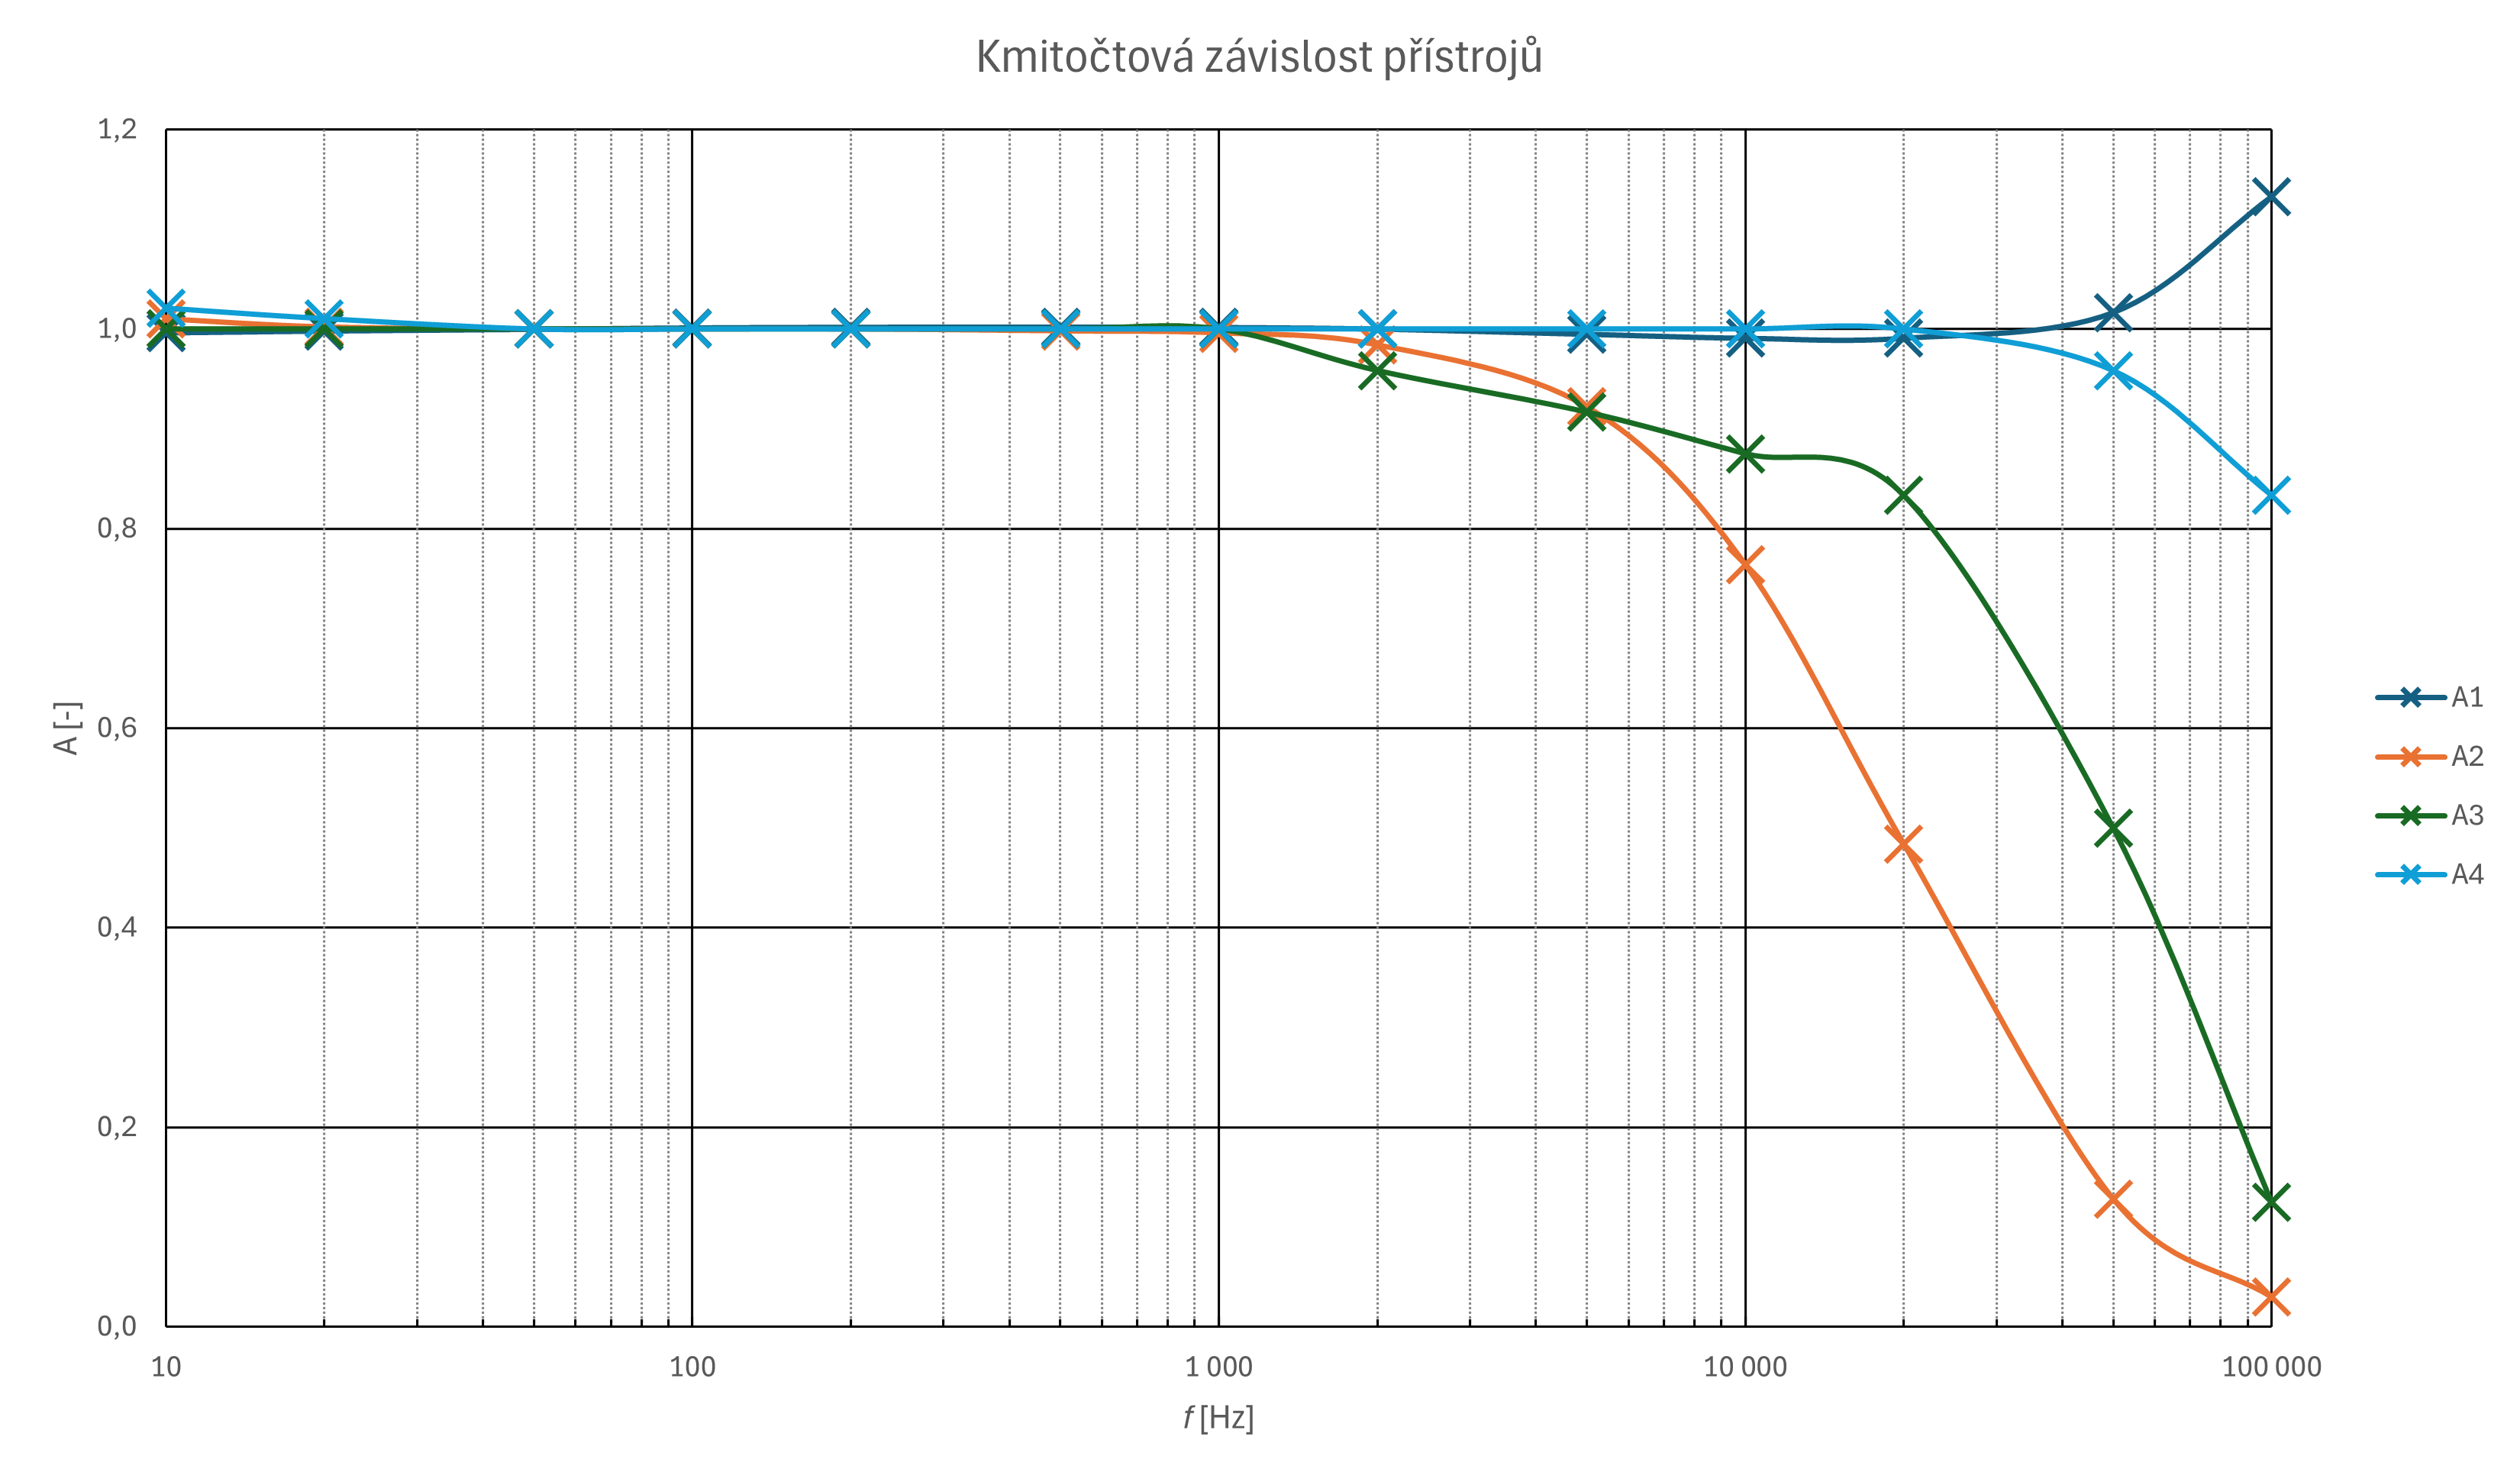
\includegraphics[width=\textwidth]{graf1.png}
    \caption{Kmitočtová závislost přístrojů}
\end{figure}

\begin{figure}[H]
    \centering
    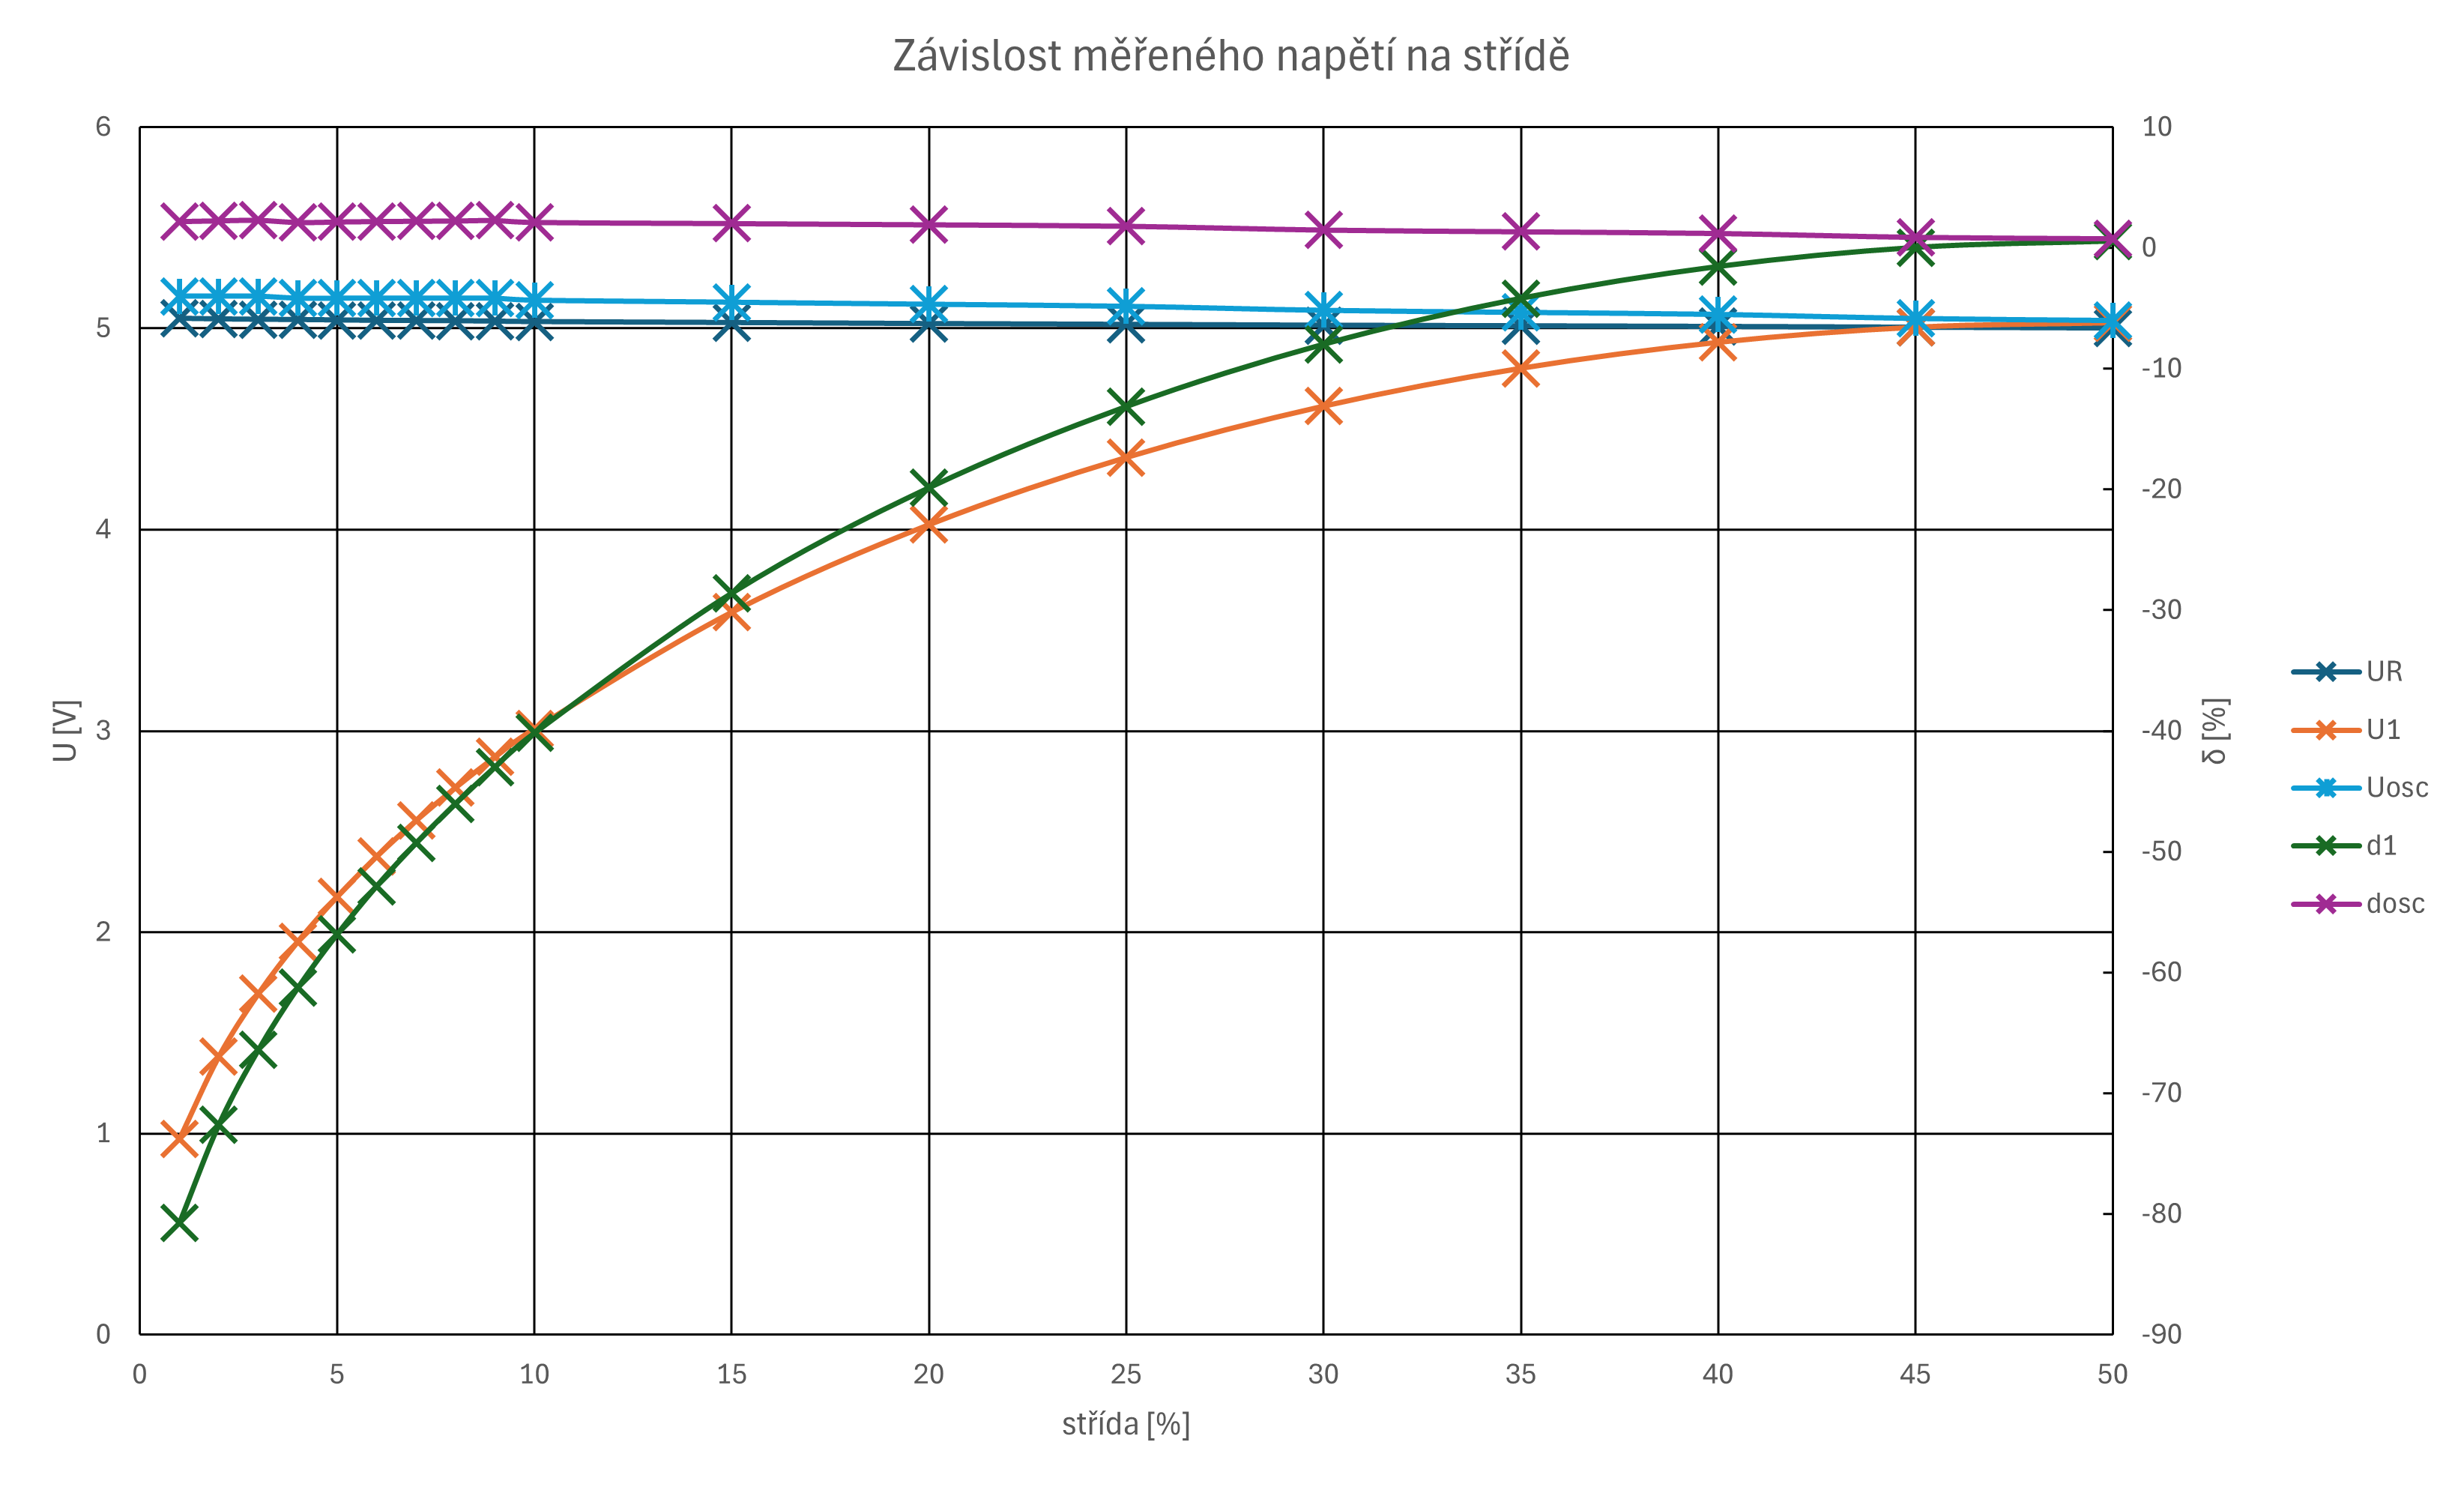
\includegraphics[width=\textwidth]{graf2.png}
    \caption{Závislost efektivní hodnoty napětí $U_1$, $U_{OSC}$, $U_R$ a relativních chyb $\delta_{OSC}$, $\delta_R$ na střídě}
\end{figure}

\pagebreak

\subsection{Příklady výpočtu}

\begin{enumerate}
    \item Kmitočtová závislost
    \begin{multline*}
        A_1 \left(f\right) = \textcolor{teal}{\frac{U \left(f\right)}{U \left(50\right)}} = \frac{U_1 \left(10\right)}{U \left(50\right)} = \frac{5,003V}{5,021V} = \underline{\underline{996,4 \cdot 10^{-3}}} \hfill
    \end{multline*}
    \item Korigovaná hodnota napětí
    \begin{multline*}
        U_{2k} = \textcolor{teal}{U_2 \cdot \frac{k_t}{k_{tH}}} = 4,81V \cdot \frac{1,155}{1,111} = \underline{\underline{5\ V}} \hfill
    \end{multline*}
    \item Relativní odchylka metody
    \begin{multline*}
        \delta_1 = \textcolor{teal}{\frac{U_1 - U}{U} \cdot 100\%} = \frac{5,022V - 5V}{5V} \cdot 100 \% = \underline{\underline{0,44\ \%}} \hfill
    \end{multline*}
    \item Korigovaná relativní odchylka
    \begin{multline*}
        \delta_{2k} = \textcolor{teal}{\frac{U_{2k} - U}{U} \cdot 100\%} = \frac{4,986 V - 5V}{5V} \cdot 100 \% = \underline{\underline{-0,27\ \%}} \hfill
    \end{multline*}
\end{enumerate}

\section{Seznam použitých přístrojů}

\begin{itemize}
    \item Laboratorní číslicový multimetr Fluke 45, v.č. 5545143
    \item Laboratorní analogový voltmetr Metra, v.č. 603629
    \item Ruční analogový multimetr Metra PU 500, v.č. 5233569
    \item Ruční číslicový multimetr UNI-T UT61A, v.č. 814019983
    \item Ruční číslicový multimetr UNI-T UT61E, v.č. 814020112
    \item Číslicový signálový generátor Siglent SDG-2042X, v.č. SDG2XCAC2T0580
    \item Číslicový osciloskop Agilent DSO-X 3014A, v.č. MY51290284
\end{itemize}

\section{Závěr}

Při měření kmitočtové závislosti byl nejpřesnějším měřícím přístrojem ruční číslicový multimetr UT61E, který i přesto, že výrobce uvádí pouze pro měření do 10khz, měřil poměrně přesně ažd o 50kHz.
Číslicový voltmetr UT61A měřil s přijatelnou přesností do 2kHz, i když jej výrobce určuje pouze pro rozsah 45–400Hz.
U magnetoeletrického multimetru PU 500 se hodnota napětí od počátku odchylovala od referenčního voltmetru o 0,2V, ale udržoval tuto hodnotu konzistentně až do 2 kHz, výrobce jej určuje pro měření do 1 kHz.
Toto je však způsobeno zejména stupnicí s nízkým rozlišením.
ML 10 byl kmitočtově nezávislý do 20kHz.
Tento ořístroj také jako jediný vykázal značnou výchylku při měření s nejnižší hodnotou, tedy 10 Hz.

Při použití měŕících přístrojů UT61A nebo PU 500 na měření neharmonických signálů je třeba kompenzovat nepřesnost vzniklou usměrněním signálu pomocí činitele tvaru $k_t$.

Při měření napětí s nenulovou stejnosměrnou složkou se i po započítání činitele tvaru jako jediný vhodný přístroj pro toto měření ukázal multimetr PU 500. Přístroje UT61A a UT61E nebyly schopny měřit obě složky signálu současně.

Pro měření obdélníkové signálu s různými poměry střídy správně měřil pouze a osciloskop.
Multimetr UT61E dosáhl při měření očekávané hodnoty až při hodnotě střídy 45\%.

\end{document}